\documentclass[11pt,a4paper,final]{article}

\usepackage[T1]{fontenc}
\usepackage[utf8]{inputenc}
\usepackage[italian]{babel}
\usepackage{layaureo}
\usepackage{microtype}
\usepackage{fancyhdr}

\usepackage{tikz}
\usetikzlibrary{trees}
\usepackage{graphicx}
\usepackage{hyperref}
\usepackage{caption}
\usepackage[list=true]{subcaption}
\captionsetup{tableposition=top, figureposition=bottom, font=small}

% tabelle
\usepackage{booktabs}
\usepackage{multirow}
\usepackage{siunitx}
\sisetup{output-decimal-marker={,}}

\usepackage{xspace}
\usepackage{rotating}

\definecolor{redUni}{RGB}{181,18,27}

% dati documento
\author{Marco Pezzutti - 1084411}
\title{CPLEX e Tabu Search}
\date{}

% macro
\def\campo#1{\uppercase{\textit{#1}}\xspace}
\def\acronimo#1{\uppercase{#1}\xspace}
\def\script#1{\texttt{#1}\xspace}
\def\modo#1{\uppercase{#1}\xspace}
\def\comando#1{\uppercase{\texttt{#1}}\xspace}

\def\memoclong{\textit{Metodi e Modelli per l'Ottimizzazione Combinatoria}\xspace}
\def\memoc{\textit{MeMOC}\xspace}
\def\tabu{\textit{Tabu Search}\xspace}

% stile pagina
\pagestyle{fancy}
\renewcommand{\headrulewidth}{0pt}
\fancyhead[RE, LO]{}
\fancyfoot{}
\fancyfoot[RO, LE]{\thepage{}}
\fancyfoot[RE, LO]{Esercitazione di \memoc}
\renewcommand{\footrulewidth}{0.4pt}

\begin{document}
\begin{titlepage}
\begin{center}

\includegraphics[width=40mm]{immagini/Logo_Padova.png}\\[1cm]
\textcolor{redUni}{\textsc{\LARGE Università degli Studi di Padova}}\\[0.5cm]
\textcolor{redUni}{\textsc{\Large Dipartimento di Matematica}}\\[0.5cm]
\textcolor{redUni}{\textsc{\Large Corso di Laurea Magistrale in Informatica}}\\[2cm]
\textsc{\Large Esercitazione di Metodi e Modelli per l'Ottimizzazione Combinatoria}\\[0.5cm]
\textsc{\large Anno 2014-2015} \\[1cm]
\rule{\linewidth}{0.3mm}\\[0.5cm]
{\huge \bfseries CPLEX e Tabu Search}\\[0.3cm]
\rule{\linewidth}{0.3mm}\\[1cm]
\begin{minipage}{0.4\textwidth}
	\begin{flushleft}
	\emph{Autore:}\\
	\textsc{\large Pezzutti Marco}\\
	\end{flushleft}
\end{minipage}
\begin{minipage}{0.4\textwidth}
	\begin{flushright}
	\emph{Matricola:}\\
	\textsc{\large 1084411}\\
	\end{flushright}
\end{minipage}
\end{center}
\end{titlepage}

\tableofcontents
\listoffigures
\listoftables
\newpage

\section{Introduzione}
Con la presente relazione intendo descrivere in modo dettagliato il lavoro svolto per completare le esercitazioni dell'insegnamento \memoclong. In particolare descriverò come ho implementato il modello di programmazione matematica fornito per il problema della foratura di pannelli attraverso le \acronimo{api} di \acronimo{cplex}, come ho generato le istanze di prova per effettuare i test e illustrerò i risultati ottenuti tramite dei grafici esplicativi.

Per quanto riguarda la seconda esercitazione, ho deciso di implementare la metaeuristica \tabu in quanto mi è sembrato essere un metodo di risoluzione interessante da sviluppare. Per effettuare i test su questo algoritmo ho utilizzato gli stessi problemi generati per la prima parte, in modo da poter effettuare un confronto prestazionale coerente tra le due tecniche.

Ho quindi disegnato dei grafici per valutare la bontà della mia implementazione con diversi valori di \emph{tabu tenure} e confrontato poi i risultati ottenuti con quelli relativi all'implementazione con \acronimo{cplex}.
%\clearpage
\section{Strumenti utilizzati}
Per la realizzazione delle esercitazioni mi sono avvalso di diversi strumenti e linguaggi di programmazione: alcuni usati per l'effettiva implementazione dei metodi e altri per automatizzare le procedure di creazione delle istanze, della loro risoluzione e della realizzazione dei grafici.
Di seguito verranno descritti gli strumenti che ho utilizzato e le motivazioni che mi hanno guidato nella loro scelta.

\begin{description}
	\item[\textsc{C$++$}]: linguaggio di programmazione orientato agli oggetti che ho utilizzato per l'implementazione del modello per la risoluzione mediante applicativo \acronimo{cplex} e per lo sviluppo della metaeuristica \tabu;
	\item[\textsc{Make}]: per automatizzare il processo di compilazione dei sorgenti e generazione dei file eseguibili sono stati utilizzati due \emph{makefile} diversi, uno per esercitazione;
	\item[\textsc{CPLEX}]: software di ottimizzazione implementato nel linguaggio \acronimo{C} in grado di risolvere problemi di programmazione lineare e lineare intera utilizzando le varianti primale e duale del metodo del simplesso insieme a metodi di \emph{Branch and Bound}. Fornisce delle \acronimo{api} verso diversi linguaggi, tra cui il \acronimo{c$++$};
	\item[\textsc{Python}]: linguaggio multiparadigma, semplice e flessibile che consente di sviluppare script in poco tempo e, grazie alla notevole quantità di librerie esistenti, consente di scrivere anche applicazioni complesse.
	
	Ho utilizzato questo linguaggio per la creazione delle istanze del problema in quanto non era pensabile produrre a mano un numero ragionevole di problemi; inoltre è stato utilizzato per analizzare i risultati ottenuti e produrre i dati statistici da visualizzare sui grafici;
	\item[\textsc{Gnuplot}]: programma che consente di disegnare grafici mediante l'utilizzo di funzioni matematiche o di dati grezzi sia in \acronimo{2d} che in \acronimo{3d}; è semplice da utilizzare ma è dotato di molte opzioni per personalizzare la resa dei grafici e la visualizzazione dei dati;
	\item[\textsc{Bash}]: per rendere automatici i processi di creazione delle istanze, di risoluzione mediante i due algoritmi e di analisi dei dati, ho realizzato uno script bash che tramite diverse opzioni consente di eseguire le operazioni desiderate.
\end{description}

\subsection{Ambiente di sviluppo}
\label{sec:ambiente}
I programmi sono stati sviluppati sul notebook in mio possesso dotato delle seguenti caratteristiche hardware:
\begin{description}
\item[\textsc{processore}]: Intel Core i7-2670QM @ 2.20GHz
\item[\textsc{ram}]: 8\acronimo{gb}
\end{description}

Di seguito sono riportate le versioni di software, linguaggi e librerie utilizzate:
\begin{description}
\item[\textbf{C$++$}]: \acronimo{c$++$03}
\item[\textbf{Make}]: 4.1
\item[\textbf{CPLEX}]: 12.6.0
\item[\textbf{Python}]: 3.5.0
\item[\textbf{Gnuplot}]: 5.0
\item[\textbf{Bash}]: 4.3.42
\end{description}

I programmi sviluppati sono stati testati anche presso la macchina del laboratorio disponibile mediante \emph{ssh} all'indirizzo \script{torre.studenti.math.unipd.it} e sono quindi conformi alle specifiche date.
%\clearpage
\section{Sviluppo}
Lo sviluppo del codice è stato diviso in due fasi distinte, la prima ha riguardato l'implementazione del modello del problema in \acronimo{cplex}, lo sviluppo degli script \emph{Python} per la generazione delle istanze e l'analisi dei dati, la produzione dei grafici; in un secondo momento ho affrontato la progettazione e lo sviluppo della \tabu per poi integrare il codice prodotto nel processo di automazione precedentemente creato.

Per ragioni di semplicità espositiva non verranno analizzati in dettaglio ogni classe e metodo sviluppati, per avere una visione particolareggiata si può ricorrere alla lettura diretta del codice che presenta una documentazione sufficiente a comprenderne il funzionamento.

Vengono quindi descritte prima le parti principali delle implementazioni degli algoritmi usati; in seguito verranno descritti gli script di utilità creati a supporto dei programmi veri e propri.

\subsection{Cplex}
Per la realizzazione della prima esercitazione, e quindi dell'implementazione del modello di programmazione mediante le \acronimo{api} di \acronimo{cplex}, è stata mantenuta la struttura del codice fornita durante i laboratori, con l'aggiunta di una classe.
I file coinvolti sono \script{pannello.h}, \script{pannello.cpp} che riguardano la nuova classe aggiunta, \script{cpxmacro.h} che riguarda delle macro utili al funzionamento di \acronimo{cplex} e \script{main.cpp}:

\begin{description}
	\item[\textsc{Pannello}]: classe progettata per rappresentare un'istanza del problema, possiede infatti attributi che indicano il numero di nodi, la matrice dei costi e l'identificativo di ogni nodo;
	\begin{description}
		\item[\textsc{readFile}]: metodo che consente di leggere il file di input, che contiene i valori relativi all'istanza generata, e di inizializzare gli attributi dell'oggetto;
	\end{description}
	\item[\textsc{main}]: metodo principale che inizializza \acronimo{cplex} preparando l'ambiente, che calcola i tempi di esecuzione e scrive i risultati ottenuti su file;
	\item[\textsc{setupLP}]: metodo che implementa il modello di programmazione matematica del problema; vengono definite prima le variabili presenti e, in seguito, vengono inseriti i vincoli in modo da permettere all'ottimizzatore di risolvere il problema.
\end{description}

Per la risoluzione del problema ho deciso di adottare il modello di \acronimo{tsp} asimmetrico trasformando il grafo del problema, che per natura sarebbe non orientato, in un grafo orientato, utilizzando due archi con lo stesso peso per ogni spigolo.

Inizialmente ho definito delle variabili intere che rappresentano le unità di flusso trasportate tra due nodi diversi e delle variabili binarie che identificano l'utilizzo o meno di un arco nella soluzione.
Ho quindi inserito il vincolo di flusso sul nodo di partenza, i vincoli di bilanciamento di flusso sui restanti nodi, i quali indicano che la quantità di flusso entrante deve corrispondere a quella uscente, due serie di vincoli che indicano che deve esistere un solo arco uscente ed un solo arco entrante per nodo e infine i vincoli che mettono in relazione le variabili del problema.

\subsection{Tabu Search}
La \tabu è un metodo basato sulla ricerca locale in grado di superare il limite dei minimi locali sfruttando meccanismi di memoria: con tale metodo si cerca di sfruttare la struttura dello spazio di ricerca memorizzando alcune informazioni sulle soluzioni già visitate in modo da orientare la ricerca ed evitare di incappare in cicli.

Per raggiungere l'obiettivo la metaerusitica fa uso di una \emph{tabu list}: struttura dati dove vengono salvate le ultime mosse effettuate; una mossa identifica i cambiamenti apportati alla soluzione corrente per giungere alla prossima soluzione esplorata.

L'implementazione della \tabu ha richiesto una fase di progettazione iniziale dove ho definito classi e metodi da utilizzare, ho cercato di sviluppare un codice il più possibile modulare; ne è scaturita la seguente struttura che per semplicità espositiva non scenderà nei minimi dettagli in quanto il codice allegato è ben documentato:

\begin{description}
	\item[\textsc{Istanza}]: classe che rappresenta un'istanza del problema, possiede come attributi la matrice dei costi e il numero di nodi del problema;
	\begin{description}
		\item[\textsc{readFile}]: metodo usato per leggere i dati del problema da file;
		\item[\textsc{maxCosto}]: metodo che calcola il costo massimo tra due nodi;
		\item[\textsc{minCosto}]: metodo che cerca i due nodi tra i quali inserire a costo minimo un terzo nodo;
	\end{description}
	\item[\textsc{Soluzione}]: classe che rappresenta la soluzione al problema utilizzando la \emph{path representation}, ovvero un vettore con la sequenza di nodi che costituiscono il ciclo di costo minimo.
	\begin{description}
		\item[\textsc{shuffleCosto}]: metodo usato per ottenere una soluzione di partenza casuale;
		\item[\textsc{invertiSequenza}]: metodo usato per invertire una sottosequenza della soluzione compresa tra due nodi;
		\item[\textsc{calcolaCosto}]: metodo usato per calcolare il costo della soluzione corrente;
		\item[\textsc{calcolaCostoVicino}]: metodo usato per calcolare il costo del vicino;
		\item[\textsc{stampa}]: metodo usato per stampare la soluzione corrente;
	\end{description}
	\item[\textsc{Mossa}]: classe che rappresenta una mossa effettuata, indica cioè i nodi iniziale e finale della sottosequenza invertita; possiede come attributi il nodo di partenza e arrivo e il costo della soluzione che si ottiene effettuando la mossa;
	\begin{description}
		\item[\textsc{operator==}]: è stato ridefinito l'operatore di uguaglianza in modo da rendere semplici i confronti tra due mosse;
	\end{description}
	\item[\textsc{Solutore}]: classe che si occupa di risolvere l'istanza del problema ottenendo una soluzione e stampandola su file;
	\begin{description}
		\item[\textsc{istanza}]: riferimento all'istanza corrente;
		\item[\textsc{soluzione}]: riferimento alla soluzione corrente;
		\item[\textsc{tabuList}]: vettore delle mosse tabu;
		\item[\textsc{mosseMigliori}]: insieme delle mosse che portano ai vicini con costo migliore;
		\item[\textsc{tabuSearch}]: metodo principale che risolve il problema dato implementando la metaeuristica \tabu;
		\item[\textsc{startSoluzione}]: metodo che determina la soluzione di partenza del problema;
		\item[\textsc{trovaVicini}]: metodo che effettua la ricerca del vicinato e salva i vicini migliori;
		\item[\textsc{scegliVicino}]: metodo che sceglie il vicino sul quale spostarsi;
		\item[\textsc{controllaMossa}]: metodo che controlla se una mossa è presente nella \emph{tabu list};
		\item[\textsc{inserisciMossaTabu}]: metodo che aggiunge la mossa effettuata alla \emph{tabu list};
	\end{description}
\end{description}

Essendo un metodo di ricerca generico, la \tabu richiede di essere specializzata per risolvere uno specifico problema.
Di seguito vengono elencate le componenti del metodo che necessitano di questa specializzazione:

\begin{description}
\item[\textsc{Soluzione}]:
\item[\textsc{Vicinato}]:
\item[\textsc{Mosse}]:
\item[\textsc{Strategia esplorazione}]:
\item[\textsc{Soluzione di partenza}]:
\item[\textsc{Condizioni di terminazione}]:
\end{description}

L'implementazione della metaeuristica \tabu, e della ricerca locale di cui fa uso, richiede di effettuare alcune scelte su come rappresentare la soluzione e di conseguenza la definizione del vicinato e delle mosse per spostarsi al suo interno. È necessario inoltre scegliere la strategia di esplorazione dei vicini, la determinazione della soluzione di partenza e le condizioni di terminazione.

Io ho scelto di adottare la \emph{path representation}, come suggerito dalle dispense, un vicinato \emph{2-opt} che consente di avere un vicino per ogni coppia di nodi $i, j$ tali che $i$ precede $j$ nella sequenza centro del vicinato.

Ho scelto, inoltre, di adottare come strategia di esplorazione la \emph{steepest descent} utilizzando però due varianti diverse, in un caso viene scelto il vicino migliore, nell'altro viene scelto casualmente un vicino tra i migliori trovati.

Anche per quanto riguarda la soluzione di partenza ho adottato due tecniche diverse, la prima è la \emph{Farthest Insertion} che crea il ciclo iniziale inserendo i nodi più distanti e continua cercando il nodo più lontano tra quelli non ancora inseriti, aggiungendolo tra due nodi consecutivi per cui è minimo il costo di inserimento.

La condizione di terminazione che ho scelto è basata sul numero massimo di iterazioni dell'algoritmo e non ho implementato alcun criterio di aspirazione in quanto da alcune prove iniziali non mi è sembrato portasse benefici alla mia implementazione.

\subsection{Script \emph{Python}}
\subsubsection{generator.py}
Lo script \script{generator.py} è stato creato per agevolare la generazione di istanze di problemi da risolvere con i due metodi scelti; è stato progettato per essere eseguito con diverse opzioni e parametri in modo da soddisfare tutte le esigenze dell'utente; di seguito viene descritta la struttura principale e le funzionalità fornite:

\begin{description}
	\item[\textsc{Node}]: classe che rappresenta un foro sulla griglia, possiede attributi di posizione $(x, y)$ e un numero identificativo;
	\item[\textsc{Grid}]: classe che rappresenta un pannello sul quale vengono fatti i fori; in pratica è costituito da una griglia a due dimensioni sul quale vengono collocati i nodi.
	\begin{description}
		\item[\textsc{manhattan\_distance}]: metodo utilizzato per calcolare la distanza tra due nodi sulla griglia sfruttando la distanza Manhattan\footnote{\url{http://it.wikipedia.org/wiki/Geometria_del_taxi}};
		\item[\textsc{print\_file}]: metodo che genera due file, uno con la configurazione della griglia e uno con la matrice dei costi per essere letto da \acronimo{CPLEX};
	\end{description}
	\item[\textsc{Generator}]: classe che rappresenta il generatore di istanze, si occupa di creare i nodi e di inserirli nella griglia;
	\begin{description}
		\item[\textsc{crea\_nodi}]: metodo che crea i nodi con tre diverse modalità: distribuzione casuale sulla griglia, distribuzione a cluster con un numero di cluster da 1 a 4 e distribuzione circolare.
	\end{description}
\end{description}

\subsubsection{statistic.py}
Lo script \script{statistic.py} è stato creato per effettuare l'analisi dei dati ottenuti mediante l'esecuzione dei metodi di risoluzione producendo poi le medie e le deviazioni standard per disegnare i grafici.

Lo script possiede un'unica classe che si occupa di svolgere tutto il lavoro:
\begin{description}
	\item[\textsc{Data}]: classe che che legge i risultati, calcola le statistiche sugli stessi e scrive i dati su file;
	\begin{description}
		\item[\textsc{read\_data[\_tabu]}]: metodo che si occupa di leggere i dati da file e calcola medie e deviazioni standard;
		\item[\textsc{write\_data[\_tabu]}]: metodo che si occupa di scrivere le statistiche su file per essere elaborati da \emph{Gnuplot}.
	\end{description}
\end{description}

\subsection{Script \emph{Gnuplot}}
Per la stampa dei grafici riguardanti i tempi di risoluzione e i costi con i relativi confronti tra algoritmi, è stato creato uno script chiamato \script{plot.gnuplot} che ha il compito di produrre i file in formato \acronimo{pdf} che verranno poi aggiunti a questa relazione.

\subsection{Script \emph{Bash}}
\label{sec:bash}
Lo script \emph{Bash} denominato \script{eserc\_lab.sh} è stato creato con il preciso scopo di automatizzare i processi di creazione, elaborazione e stampa dei dati e per fornire all'utente uno strumento per eseguire solo alcune attività in modo mirato.

Di seguito vengono elencate le principali funzioni dello script, vengono tralasciate funzionalità accessorie quali la creazione delle cartelle e file, le impostazioni delle variabili e la rimozione di vecchi risultati:

\begin{description}
	\item[\textsc{crea\_casuali}]: funzione che richiama lo script \script{generator.py} indicando quante istanze creare, quanti nodi, quale dimensione della griglia per generare istanze casuali;
	\item[\textsc{crea\_cluster}]: funzione che richiama lo script \script{generator.py} indicando quante istanze creare, quanti nodi, quale dimensione della griglia e quanti cluster per generare istanze a cluster;
	\item[\textsc{crea\_circolari}]: funzione che richiama lo script \script{generator.py} indicando quante istanze creare, quanti nodi, quale dimensione della griglia per generare istanze circolari;
	\item[\textsc{risolvi\_cplex}]: funzione che richiama il programma \script{cplex} una volta per ogni istanza generata, passando come parametri il nome del file relativo al problema e il numero di problema;
	\item[\textsc{risolvi\_tabu}]: funzione che richiama il programma \script{tabusearch} una volta per ogni istanza casuale generata, passando come parametri il nome del file relativo al problema, il numero di problema, il valore della tabu tenure e il numero massimo di iterazioni da effettuare;
	\item[\textsc{calcola\_statistiche}]: funzione che richiama lo script \script{statistic.py} per l'analisi dei risultati;
	\item[\textsc{crea\_grafici}]: funzione che richiama lo script \script{plot.gnuplot} per la generazione dei grafici.
\end{description}
%\clearpage
\section{Esecuzione}
L'esecuzione del programma è gestita mediante lo script \emph{bash} chiamato \script{eserc\_lab.sh}; tale script è stato dotato di diverse opzioni che permettono di eseguire il programma con diverse modalità richiamabili tramite gli appositi flag:

\begin{description}
	\item[\texttt{-a arg}]: modalità \modo{all}, esegue in sequenza tutte le operazioni descritte nella sezione \ref{sec:bash} e comprende tutte le altre modalità di esecuzione; permette quindi di eseguire l'intero programma ed ottenere tutti i risultati; l'argomento \texttt{arg} è necessario per impostare il numero di istanze da generare in quanto indica il numero di ripetizioni da effettuare;
	\item[\texttt{-c arg}]: modalità \modo{casuali}, richiama lo script \script{generator.py} per generare solamente i problemi creati casualmente; l'argomento \texttt{arg} serve per impostare il numero di problemi da generare;
	\item[\texttt{-g}]: modalità \modo{gnuplot}, richiama \emph{gnuplot} per disegnare i grafici con i dati ottenuti;
	\item[\texttt{-i arg}]: modalità \modo{circolari}, richiama lo script \script{generator.py} per generare  solamente i problemi circolari; l'argomento \texttt{arg} serve per impostare il numero di problemi da generare;
	\item[\texttt{-l arg}]: modalità \modo{cluster}, richiama lo script \script{generator.py} per generare  solamente i problemi a cluster; l'argomento \texttt{arg} serve per impostare il numero di problemi da generare;
	\item[\texttt{-r arg}]: modalità \modo{cplex}, richiama il programma \script{cplex} per risolvere i problemi che sono stati generati; l'argomento \texttt{arg} serve per indicare il numero di problemi da risolvere;
	\item[\texttt{-s}]: modalità \modo{statistiche}, richiama lo script \script{statistic.py} per elaborare i risultati ottenuti e generare i file di input per \emph{gnuplot};
	\item[\texttt{-t arg}]: modalità \modo{tabu search}, richiama il programma \script{tabusearch} per risolvere i problemi generati; l'argomento \texttt{arg} serve per indicare il numero di problemi da risolvere.
\end{description}

Per valutare e confrontare l'efficienza dei due metodi in modo significativo è necessario avere una considerevole quantità di dati, questo implica il dover generare e risolvere molte istanze diverse.

Per questo motivo ho deciso di creare tre diversi tipi di problemi: istanze con distribuzione di nodi casuale all'interno della griglia, con una disposizione a cluster, suddividendo la griglia in quarti e concentrando la disposizione dei nodi prima su un quarto, poi su due, tre e quattro cluster in modo da capire se ci sono differenze a parità di densità di nodi: ho utilizzato infatti come indice per creare i nodi la densità in funzione delle dimensioni della griglia, o del cluster.

Come ultima tipologia di istanza ho usato quella circolare che, su una griglia con nodi equispaziati, equivale ad un quadrato con i vertici in direzione degli assi dei lati della griglia stessa.

Una volta creati i nodi, per calcolare il peso degli archi che li unisce ho utilizzato la distanza Manhattan.



\subsection{Struttura cartelle}
Affinché l'esecuzione dei programmi non provochi errori è necessario che la struttura di file sia coerente con quella usata nell'ambiente di sviluppo; insieme alla presente relazione viene fornito un archivio contenente tutti i file sviluppati necessari al funzionamento, tralasciando, ovviamente, quelli che verranno creati dagli stessi programmi.

Qui di seguito viene descritta la struttura di file e cartelle nell'ambiente di sviluppo:\\*

%disegna la struttura di cartelle presente nell'archivio consegnato
\tikzstyle{every node}=[thick,anchor=west, rounded corners, font={\scriptsize\ttfamily}, inner sep=2.5pt]
\tikzstyle{selected}=[draw=blue,fill=blue!10]
\tikzstyle{root}=[selected, fill=blue!30]
\tikzstyle{optional}=[dashed, draw=blue, fill=blue!5]

\begin{tikzpicture}[%
    scale=.6,
    grow via three points={one child at (0.5,-0.65) and
    two children at (0.5,-0.65) and (0.5,-1.1)},
    edge from parent path={(\tikzparentnode.south) |- (\tikzchildnode.west)}]
  \node [root] {eserc.lab.01}
    child { node at (10,0) [selected] {eserc.lab.02}
      child { node {istanza.cpp}}
      child { node {istanza.cpp}}
      child { node {main.cpp}}
      child { node {Makefile}}
      child { node {mossa.cpp}}
      child { node {mossa.h}}
      child { node {solutore.cpp}}
      child { node {solutore.h}}
      child { node {soluzione.cpp}}
      child { node {soluzione.h}}
    }
    child { node at (5,-0.5) [optional] {instances}
    }
    child { node at (5,-0.9) [optional] {results}
    }
    child { node at (5,-1.3) [optional] {solutions}
    }
    child { node at (0,-1.5) {cpxmacro.h}}
    child { node at (0,-1.7) {eserc\_lab.sh}}
    child { node at (0,-1.9) {generator.py}}
    child { node at (0,-2.1) {main.cpp}}
    child { node at (0,-2.3) {Makefile}}
    child { node at (0,-2.5) {pannello.cpp}}
    child { node at (0,-2.7) {pannello.h}}
    child { node at (0,-2.9) {plot.gnuplot}}
    child { node at (0,-3.1) {statistic.py}};
\end{tikzpicture}


\subsection{Compilazione}
Una volta aperto l'archivio contenente il codice sorgente ed essersi assicurati che siano installati e presenti nella variabile di sistema \comando{path} le librerie e i software descritti nella sezione \ref{sec:ambiente} e, prima di eseguire il programma tramite script \emph{bash}, è necessario procedere alla compilazione del codice \acronimo{c$++$}: per fare questo è sufficiente digitare ed eseguire il comando \script{make} all'interno della cartella radice del progetto, per compilare \script{cplex}, ed eseguire nuovamente il comando \script{make} all'interno della cartella \script{eserc.lab.02} per compilare \script{tabusearch}.


%\clearpage
\section{Risultati}
\label{sec:risultati}
I programmi sono stati eseguiti mediante il seguente comando:
\begin{quotation}
\script{bash eserc\_lab.sh -a 20}
\end{quotation}
che esegue l'intero processo, generando 20 problemi simili per ogni incremento della densità dei nodi, pari a $10$, per le istanze \emph{casuali} e \emph{cluster}; mentre vengono generati solamente 20 problemi con istanze \emph{circolari} in quanto non è presente casualità nella loro generazione.

In totale sono quindi state generate $1020$ istanze, $200$ di tipo casuale, $800$ di tipo cluster e $20$ di tipo circolare.

I grafici riportano sull'asse delle ascisse il numero di nodi del problema, mentre sull'asse delle ordinate il tempo in secondi che è servito per trovare la soluzione, da notare che si è scelto di rappresentare il tempo in scala logaritmica.

I punti di interesse sono quelli identificati dal simbolo presente nella legenda di ogni grafico e rappresentano la media dei risultati ottenuti per le istanze simili, mentre le linee verticali indicano la variabilità nei risultati individuata tramite la deviazione standard.

\subsection{\acronimo{cplex}}
\begin{figure}[htb]
	\centering
	\begin{subfigure}[b]{.45\textwidth}
		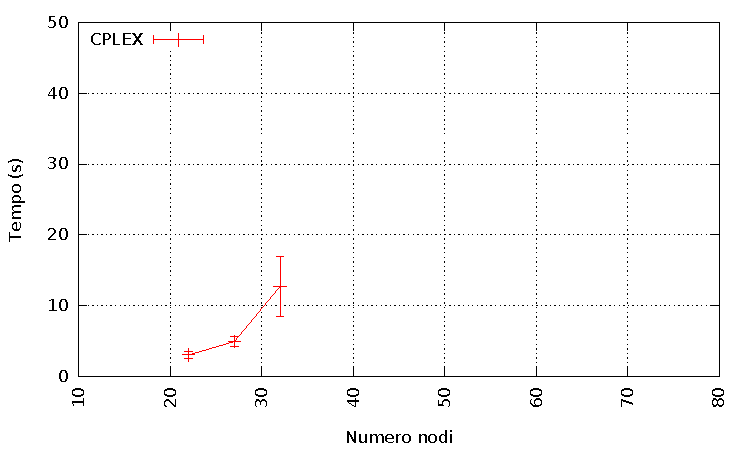
\includegraphics[width=\textwidth]{immagini/cplex_casuali.pdf}
		\caption{Istanze casuali}
		\label{fig:casuali cplex}
	\end{subfigure}
	\quad
	\begin{subfigure}[b]{.45\textwidth}
		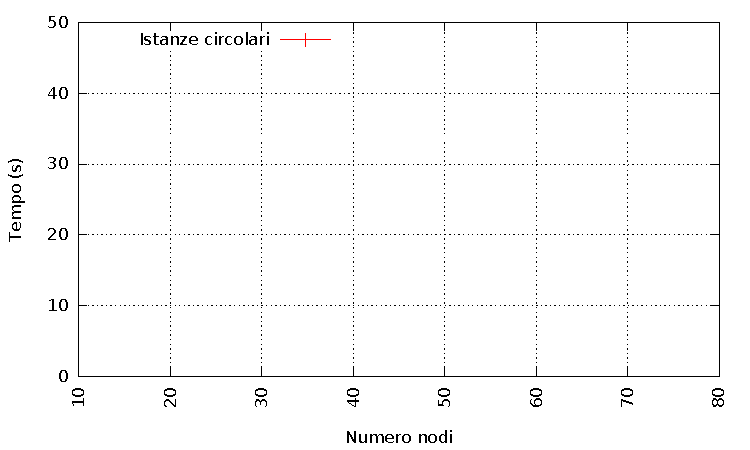
\includegraphics[width=\textwidth]{immagini/cplex_circolari.pdf}
		\caption{Istanze circolari}
		\label{fig:circolari cplex}
	\end{subfigure}
	\caption{Istanza casuali e circolari - \acronimo{cplex}}
	\label{fig:casuali circolari cplex}
\end{figure}

In figura \ref{fig:casuali cplex} vediamo i risultati per le istanze casuali, esse seguono un andamento abbastanza regolare con il crescere del numero dei nodi: per istanze piccole il tempo di risoluzione è abbastanza rapido, ma sale molto velocemente, fino a oltre $200s$, con l'aumentare dei nodi.

\begin{table}[htb]
	\footnotesize
	\centering
	\caption{Tempi e costi istanze casuali - \acronimo{cplex}}
	\label{tab:casuali}
	\begin{tabular}{cS[table-format=3.4]S[table-format=2.4]S[table-format=2.1]}
	\toprule
	\multirow{2}*{Numero nodi} 	& {Tempo medio} & {Deviazione standard} & \multirow{2}*{Costo medio} \\
								& {(s)}			& {(s)} 				& \\
	\midrule
	11	& 0.2438		& 0.1045	& 55.9 \\
	16	& 0.8337		& 0.3740	& 65.1 \\
	20	& 2.2390		& 1.6470	& 69.6 \\
	25	& 3.6030		& 1.2315	& 76.5 \\
	29	& 6.8557		& 3.9426	& 83.6 \\
	34	& 24.7649		& 13.2507	& 88.9 \\
	38	& 51.4854		& 25.8351	& 91.3 \\
	43	& 101.6627		& 33.2080	& 99.1 \\
	47	& 144.4995		& 24.6324	& 102.2 \\
	52	& 255.3258		& 65.0774	& 107.1 \\
	\bottomrule
	\end{tabular}
\end{table}

Per quanto riguarda le istanze circolari, vediamo in figura \ref{fig:circolari cplex} che i tempi sono molto più bassi, rispetto alle istanze casuali, con un alto numero di nodi: questo è dovuto alla semplicità intrinseca di queste istanze che sono quindi più facili da risolvere.
Da notare come l'andamento del grafico non sia molto lineare: questo fatto probabilmente è dovuto al carico del processore al momento dell'esecuzione del test, che può non essere stato costante durante il periodo di prova.

\begin{table}[htb]
	\footnotesize
	\centering
	\caption{Tempi e costi istanze circolari - \acronimo{cplex}}
	\label{tab:circolari}
	\begin{tabular}{cS[table-format=1.4]S[table-format=3.0]}
	\toprule
	\multirow{2}*{Numero nodi} 	& {Tempo medio} & \multirow{2}*{Costo} \\
								& {(s)}			&  \\
	\midrule
	8	& 0.1228	& 16 \\
	12	& 0.1209	& 24 \\
	16	& 0.0663	& 32 \\
	20	& 0.2185	& 40 \\
	24	& 0.3220	& 48 \\
	28	& 0.2246	& 56 \\
	32	& 0.4750	& 64 \\
	36	& 0.8386	& 72 \\
	40	& 1.8196	& 80 \\
	44	& 1.2220	& 88 \\
	48	& 1.2384	& 96 \\
	52	& 2.3079	& 104 \\
	56	& 4.1274	& 112 \\
	60	& 4.6480	& 120 \\
	64	& 3.7191	& 128 \\
	68	& 3.6495	& 136 \\
	72	& 3.7701	& 144 \\
	76	& 3.4811	& 152 \\
	80	& 4.2138	& 160 \\
	84	& 6.5727	& 168 \\
	\bottomrule
	\end{tabular}
\end{table}

Tutti i tempi ei costi medi ottenuti sono visibili nella tabella \ref{tab:casuali} per le istanze casuali e in tabella \ref{tab:circolari} per quelle circolari.

\begin{figure}[htb]
	\centering
	\begin{subfigure}[b]{.45\textwidth}
		\includegraphics[width=\textwidth]{immagini/cplex_cluster_1.pdf}
		\caption{Istanze 1 cluster}
	\end{subfigure}
	\quad
	\begin{subfigure}[b]{.45\textwidth}
		\includegraphics[width=\textwidth]{immagini/cplex_cluster_2.pdf}
		\caption{Istanze 2 cluster}
	\end{subfigure}
	\\
	\begin{subfigure}[b]{.45\textwidth}
		\includegraphics[width=\textwidth]{immagini/cplex_cluster_3.pdf}
		\caption{Istanze 3 cluster}
	\end{subfigure}
	\quad
	\begin{subfigure}[b]{.45\textwidth}
		\includegraphics[width=\textwidth]{immagini/cplex_cluster_4.pdf}
		\caption{Istanze 4 cluster}
	\end{subfigure}
	\caption{Istanze cluster - \acronimo{cplex}}
	\label{fig:cluster cplex}
\end{figure}

In figura \ref{fig:cluster cplex} sono riportati i grafici riguardanti le istanze cluster: si può notare come abbiano tutti un andamento simile con tempi di risoluzione comparabili eccezion fatta per le istanze con $2$ nodi a $1$ cluster che hanno richiesto un tempo molto inferiore.

L'unico aspetto da sottolineare è la deviazione standard molto alta sulle istanze con $32$ nodi a $2$ cluster che è dovuta probabilmente ad un'istanza particolare che ha richiesto un tempo di risoluzione molto superiore alle altre.

\begin{figure}[htb]
	\centering
	\includegraphics[width=\textwidth]{immagini/cplex_all.pdf}
	\caption{Istanze casuali, cluster e circolari - \script{cplex}}
	\label{fig:all cplex}
\end{figure}

Ho deciso di riportare un grafico completo di tutti i risultati ottenuti, questo è visibile in figura \ref{fig:all cplex}.
È possibile vedere come con ogni tipologia di istanza, tranne quelle circolari, a parità di numero di nodi e quindi di complessità del problema, le prestazioni del programma sono simili.

È presente solo un leggero aumento nei tempi per quanto riguarda le istanze a 2 cluster: esse infatti sono costruite utilizzando due quarti opposti della griglia, creando quindi maggiori difficoltà nella risoluzione in quanto i nodi si trovano in due zone distanti fra loro.

\begin{table}[htb]
	\footnotesize
	\centering
	\caption{Tempi e costi istanze cluster - \acronimo{cplex}}
	\label{tab:cluster}
	\begin{tabular}{ccS[table-format=3.4]S[table-format=2.4]S[table-format=2.1]}
	\toprule
		& \multirow{2}*{Numero nodi} 	& {Tempo medio} & {Deviazione standard} & \multirow{2}*{Costo medio} \\
		&								& {(s)}			& {(s)} 				& \\
	\midrule
	\multirow{10}*{\begin{sideways}1 cluster\end{sideways}} & 2	& 0.0009	& 0.0001	& 8.7 \\
	& 4	& 0.0514	& 0.0195	& 16.0 \\
	& 5	& 0.0734	& 0.0310	& 18.9 \\
	& 7	& 0.1518	& 0.0950	& 22.3 \\
	& 8	& 0.1655	& 0.1044	& 23.1 \\
	& 10	& 0.2061	& 0.1031	& 24.3 \\
	& 11	& 0.2239	& 0.0738	& 25.7 \\
	& 13	& 0.4562	& 0.2643	& 26.8 \\
	& 14	& 0.5176	& 0.1663	& 28.6 \\
	& 16	& 0.7303	& 0.4115	& 30.4 \\
	\midrule
	\multirow{10}*{\begin{sideways}2 cluster\end{sideways}} & 4	& 0.0723	& 0.0370	& 38.1 \\
	& 8	& 0.1715	& 0.0462	& 47.9 \\
	& 10	& 0.3779	& 0.1874	& 50.9 \\
	& 14	& 1.3264	& 0.6812	& 55.5 \\
	& 16	& 1.6585	& 1.0877	& 57.6 \\
	& 20	& 3.9322	& 2.1850	& 60.5 \\
	& 22	& 4.2853	& 2.8440	& 63.1 \\
	& 26	& 7.7065	& 3.8624	& 64.7 \\
	& 28	& 14.4487	& 10.7130	& 66.1 \\
	& 32	& 52.5417	& 73.9963	& 70.7 \\
	\midrule
	\multirow{10}*{\begin{sideways}3 cluster\end{sideways}} & 6	& 0.0969	& 0.0385	& 44.2 \\
	& 12	& 0.5026	& 0.2955	& 54.9 \\
	& 15	& 1.0327	& 0.6484	& 58.1 \\
	& 21	& 2.8062	& 1.7474	& 65.2 \\
	& 24	& 3.3463	& 1.3332	& 68.0 \\
	& 30	& 12.4023	& 8.0275	& 74.9 \\
	& 33	& 23.2862	& 15.1886	& 77.7 \\
	& 39	& 51.0216	& 21.6250	& 83.3 \\
	& 42	& 92.3221	& 17.6381	& 85.8 \\
	& 48	& 137.4311	& 44.2163	& 89.3 \\
	\midrule
	\multirow{10}*{\begin{sideways}4 cluster\end{sideways}} & 8	& 0.1588	& 0.1086	& 50.7 \\
	& 16	& 0.8943	& 0.4948	& 67.2 \\
	& 20	& 3.1633	& 1.9649	& 72.4 \\
	& 28	& 6.8458	& 4.1326	& 81.0 \\
	& 32	& 16.6601	& 12.6953	& 86.3 \\
	& 40	& 69.2420	& 23.0443	& 96.4 \\
	& 44	& 107.8618	& 25.5995	& 99.9 \\
	& 52	& 227.9986	& 53.9585	& 107.2 \\
	& 56	& 280.3272	& 61.0582	& 110.7 \\
	& 64	& 625.6605	& 266.3992	& 116.7 \\
	\bottomrule
	\end{tabular}
\end{table}

Nella tabella \ref{tab:cluster} sono riportati i tempi medi e i costi medi per la risoluzione delle istanze cluster.

\subsection{Tabu Search}

\begin{figure}[htb]
	\centering
	\begin{subfigure}[b]{.45\textwidth}
		\includegraphics[width=\textwidth]{immagini/tabu_4_tempo.pdf}
		\caption{Istanze casuali - tenure 4}
	\end{subfigure}
	\quad
	\begin{subfigure}[b]{.45\textwidth}
		\includegraphics[width=\textwidth]{immagini/tabu_5_tempo.pdf}
		\caption{Istanze casuali - tenure 5}
	\end{subfigure}
	\\
	\begin{subfigure}[b]{.45\textwidth}
		\includegraphics[width=\textwidth]{immagini/tabu_6_tempo.pdf}
		\caption{Istanze casuali - tenure 6}
	\end{subfigure}
	\quad
	\begin{subfigure}[b]{.45\textwidth}
		\includegraphics[width=\textwidth]{immagini/tabu_7_tempo.pdf}
		\caption{Istanze casuali - tenure 7}
	\end{subfigure}
	\\
	\begin{subfigure}[b]{.45\textwidth}
		\includegraphics[width=\textwidth]{immagini/tabu_8_tempo.pdf}
		\caption{Istanze casuali - tenure 8}
	\end{subfigure}
	\caption{Tempi istanze casuali - \tabu}
	\label{fig:tempi tabu}
\end{figure}

\begin{figure}[htb]
	\centering
	\begin{subfigure}[b]{.45\textwidth}
		\includegraphics[width=\textwidth]{immagini/tabu_4_costo.pdf}
		\caption{Istanze casuali - tenure 4}
	\end{subfigure}
	\quad
	\begin{subfigure}[b]{.45\textwidth}
		\includegraphics[width=\textwidth]{immagini/tabu_5_costo.pdf}
		\caption{Istanze casuali - tenure 5}
	\end{subfigure}
	\\
	\begin{subfigure}[b]{.45\textwidth}
		\includegraphics[width=\textwidth]{immagini/tabu_6_costo.pdf}
		\caption{Istanze casuali - tenure 6}
	\end{subfigure}
	\quad
	\begin{subfigure}[b]{.45\textwidth}
		\includegraphics[width=\textwidth]{immagini/tabu_7_costo.pdf}
		\caption{Istanze casuali - tenure 7}
	\end{subfigure}
	\\
	\begin{subfigure}[b]{.45\textwidth}
		\includegraphics[width=\textwidth]{immagini/tabu_8_costo.pdf}
		\caption{Istanze casuali - tenure 8}
	\end{subfigure}
	\caption{Costi istanze casuali - \tabu}
	\label{fig:costi tabu}
\end{figure}

\begin{figure}[htb]
	\centering
	\includegraphics[width=\textwidth]{immagini/tabu_all_tempo.pdf}
	\caption{Tempi istanze casuali - \tabu}
	\label{fig:all tempi tabu}
\end{figure}

\begin{figure}[htb]
	\centering
	\includegraphics[width=\textwidth]{immagini/tabu_all_costo.pdf}
	\caption{Costi istanze casuali - \tabu}
	\label{fig:all costi tabu}
\end{figure}

\begin{table}[htb]
	\footnotesize
	\centering
	\caption{Tempi e costi istanze casuali - \tabu}
	\label{tab:tabu}
	\begin{tabular}{cS[table-format=1.4]S[table-format=1.4]S[table-format=3.3]S[table-format=1.4]}
	\toprule
	\multirow{2}*{Numero nodi} 	& {Tempo medio} & {Deviazione standard} & \multirow{2}*{Costo medio} 	& {Deviazione standard}\\
								& {(s)}			& {(s)} 				& 								& \\
	\midrule
	11	& 0.0040	& 0.0007	& 55.9		& 5.4858 \\
	16	& 0.0110	& 0.0021	& 65.855	& 5.7060 \\
	20	& 0.0208	& 0.0027	& 70.7		& 4.3839 \\
	25	& 0.0335	& 0.0043	& 78.465	& 6.0996 \\
	29	& 0.0651	& 0.0153	& 86.41		& 5.4463 \\
	34	& 0.1149	& 0.0130	& 91.18		& 6.1521 \\
	38	& 0.1541	& 0.0046	& 94.745	& 3.1352 \\
	43	& 0.1902	& 0.0058	& 103.485	& 4.9944 \\
	47	& 0.2242	& 0.0059	& 107.55	& 3.8716 \\	
	52	& 0.2791	& 0.0065	& 113.275	& 4.1192 \\
	\midrule
	11	& 0.0044	& 0.00089	& 55.9		& 5.4858 \\
	16	& 0.0120	& 0.00151	& 65.42		& 5.4641 \\
	20	& 0.0185	& 0.00217	& 70.335	& 4.2735 \\
	25	& 0.0331	& 0.00315	& 78.065	& 5.4499 \\
	29	& 0.0599	& 0.01498	& 86.005	& 4.0309 \\
	34	& 0.1197	& 0.00567	& 91.43		& 5.7485 \\
	38	& 0.1491	& 0.00678	& 94.455	& 2.8618 \\
	43	& 0.1886	& 0.00527	& 103.07	& 5.1433 \\
	47	& 0.2281	& 0.00376	& 106.54	& 4.3268 \\
	52	& 0.2828	& 0.01059	& 112.665	& 3.7144 \\	
	\midrule
	11	& 0.0047	& 0.0010	& 55.9		& 5.4858 \\ 
	16	& 0.0114	& 0.0015	& 65.2		& 5.2475 \\
	20	& 0.0211	& 0.0034	& 70.325	& 4.1817 \\
	25	& 0.0341	& 0.0047	& 76.76		& 4.9318 \\
	29	& 0.0523	& 0.0100	& 86.13		& 5.1482 \\
	34	& 0.1183	& 0.0127	& 91.04		& 4.7051 \\
	38	& 0.1567	& 0.0052	& 94.235	& 3.8094 \\
	43	& 0.1971	& 0.0036	& 102.35	& 4.8162 \\
	47	& 0.2332	& 0.0068	& 106.45	& 4.1793 \\
	52	& 0.2878	& 0.0077	& 111.505	& 3.9733 \\
	\midrule
	11	& 0.0047	& 0.0011	& 55.9		& 5.4858 \\
	16	& 0.0118	& 0.0015	& 65.63		& 5.6266 \\
	20	& 0.0210	& 0.0017	& 69.745	& 3.9841 \\
	25	& 0.0315	& 0.0032	& 77.9		& 5.2005 \\
	29	& 0.0641	& 0.0174	& 84.46		& 4.8488 \\
	34	& 0.1217	& 0.0084	& 91.075	& 5.8853 \\
	38	& 0.1535	& 0.0078	& 93.705	& 3.1860 \\
	43	& 0.1933	& 0.0058	& 101.77	& 4.6907 \\
	47	& 0.2311	& 0.0057	& 105.8		& 4.1282 \\
	52	& 0.2846	& 0.0094	& 111.14	& 3.5792 \\
	\midrule
	11	& 0.0047	& 0.0007	& 55.9		& 5.4858 \\
	16	& 0.0120	& 0.0016	& 65.5		& 5.5772 \\
	20	& 0.0223	& 0.0024	& 70.04		& 4.1890 \\
	25	& 0.0347	& 0.0047	& 77.115	& 4.8038 \\
	29	& 0.0564	& 0.0113	& 85.115	& 5.0305 \\
	34	& 0.1251	& 0.0055	& 90.835	& 5.4048 \\
	38	& 0.1526	& 0.0051	& 94.155	& 4.1911 \\
	43	& 0.1962	& 0.0056	& 101.995	& 4.5129 \\
	47	& 0.2324	& 0.0053	& 105.55	& 3.5185 \\	
	52	& 0.2929	& 0.0080	& 110.93	& 3.7861 \\
	\bottomrule
	\end{tabular}
\end{table}
%\clearpage
\section{Conclusioni}

In figura \ref{fig:tempi cplex tabu} si può vedere come i tempi di calcolo dell'euristica \tabu per istanze casuali siano migliori di almeno due unità di grandezza rispetto a quelli ottenuti con \acronimo{cplex}: questo giustifica la perdita di precisione sui valori delle soluzioni trovati, soprattutto in contesti dove sia critico il tempo di calcolo e non sia così importante la soluzione esatta del problema.

\begin{figure}[H]
	\centering
	\includegraphics[width=.7\textwidth]{cplex_tabu_tempo}
	\caption{Tempi istanze casuali - \acronimo{cplex} vs. \tabu}
	\label{fig:tempi cplex tabu}
\end{figure}

Anche per quanto riguarda le istanze cluster, i tempi di calcolo sono a vantaggio di \tabu: si può vedere in figura \ref{fig:tempi cplex tabu cluster} che la differenza tra i 2 algoritmi è minore per le istanze a 1 cluster e con pochi nodi, ma cresce con l'aumentare dei cluster e dei nodi,  rimanendo comunque entro 2 ordini di grandezza.

\begin{figure}[H]
	\centering
	\begin{subfigure}[b]{.45\textwidth}
		\includegraphics[width=\textwidth]{cplex_tabu_cluster_1_tempo}
		\caption{Istanze 1 cluster}
	\end{subfigure}
	\quad
	\begin{subfigure}[b]{.45\textwidth}
		\includegraphics[width=\textwidth]{cplex_tabu_cluster_2_tempo}
		\caption{Istanze 2 cluster}
	\end{subfigure}
	\\
	\begin{subfigure}[b]{.45\textwidth}
		\includegraphics[width=\textwidth]{cplex_tabu_cluster_3_tempo}
		\caption{Istanze 3 cluster}
	\end{subfigure}
	\quad
	\begin{subfigure}[b]{.45\textwidth}
		\includegraphics[width=\textwidth]{cplex_tabu_cluster_4_tempo}
		\caption{Istanze 4 cluster}
	\end{subfigure}
	\caption{Tempi istanze cluster - \acronimo{cplex} vs. \tabu}
	\label{fig:tempi cplex tabu cluster}
\end{figure}

Per confrontare l'efficacia dell'implementazione della \tabu rispetto a \acronimo{cplex} ho calcolato prima la media sulle ripetizioni delle istanze identiche e poi la media sulle istanze simili con lo stesso numero di nodi ottenendo i grafici in figura \ref{fig:costi cplex tabu}: si nota che il valore della soluzione ottenuta con la metaeuristica non si allontana troppo dal valore esatto, con un basso numero di nodi, il peggioramento, si attesta intorno al $2\%$ e cresce al crescere della loro quantità.
Aumentando il valore di \emph{tabu tenure} si riesce però a mitigare la perdita di precisione recuperando circa l'$1\%$ e questo conferma la necessità di effettuare un'attenta calibrazione dei parametri con lo scopo di ottenere risultati migliori.
In figura sono riportate anche le medie dei valori peggiori delle soluzioni che sono stati calcolati con l'algoritmo e indicano come in alcuni casi la \tabu non riesca ad avvicinarsi sufficientemente all'ottimo globale incappando probabilmente in qualche ottimo locale.

\begin{figure}[H]
	\centering
	\begin{subfigure}[b]{.45\textwidth}
			\includegraphics[width=\textwidth]{cplex_tabu4_compare}
			\caption{Tabu tenure 4}
	\end{subfigure}
	\quad
	\begin{subfigure}[b]{.45\textwidth}
			\includegraphics[width=\textwidth]{cplex_tabu8_compare}
			\caption{Tabu tenure 8}
	\end{subfigure}
	\caption{Costi medi e massimi istanze casuali - \acronimo{cplex} vs \tabu}
	\label{fig:costi cplex tabu}
\end{figure}

Per quanto riguarda le istanze cluster si può osservare un comportamento simile a quello delle istanze casuali, infatti al crescere del numero di nodi e della \emph{tabu tenure} si osservano miglioramenti nei costi delle soluzioni trovate.

In particolare, per le istanze a 1 cluster (figura \ref{fig:costi cplex tabu cluster 1}), si nota che la \tabu riesce in media a trovare la soluzione ottima ma esiste una forte variabilità tra istanze simili trovando, a volte, soluzioni molto lontane da quella ottima.

\begin{figure}[H]
	\centering
	\begin{subfigure}[b]{.45\textwidth}
			\includegraphics[width=\textwidth]{cplex_tabu4_cluster1_compare}
			\caption{Tabu tenure 4}
	\end{subfigure}
	\quad
	\begin{subfigure}[b]{.45\textwidth}
			\includegraphics[width=\textwidth]{cplex_tabu8_cluster1_compare}
			\caption{Tabu tenure 8}
	\end{subfigure}
	\caption{Costi medi e massimi istanze 1 cluster - \acronimo{cplex} vs \tabu}
	\label{fig:costi cplex tabu cluster 1}
\end{figure}

Le istanze a 2 cluster (figura \ref{fig:costi cplex tabu cluster 2}) presentano anch'esse forte variabilità nel valore delle soluzioni trovate ma in media si avvicinano molto alla soluzione ottima, migliorando con l'aumentare della \emph{tabu tenure}.

\begin{figure}[H]
	\centering
	\begin{subfigure}[b]{.45\textwidth}
			\includegraphics[width=\textwidth]{cplex_tabu4_cluster2_compare}
			\caption{Tabu tenure 4}
	\end{subfigure}
	\quad
	\begin{subfigure}[b]{.45\textwidth}
			\includegraphics[width=\textwidth]{cplex_tabu8_cluster2_compare}
			\caption{Tabu tenure 8}
	\end{subfigure}
	\caption{Costi medi e massimi istanze 2 cluster - \acronimo{cplex} vs \tabu}
	\label{fig:costi cplex tabu cluster 2}
\end{figure}

Con l'aumentare dei cluster e di conseguenza dei nodi (figure \ref{fig:costi cplex tabu cluster 3} e \ref{fig:costi cplex tabu cluster 4}), si nota una costante perdita di precisione nella soluzione trovata rispetto a quella ottima, che viene mitigata con l'adozione di valori di \emph{tabu tenure} più alta.

\begin{figure}[H]
	\centering
	\begin{subfigure}[b]{.45\textwidth}
			\includegraphics[width=\textwidth]{cplex_tabu4_cluster3_compare}
			\caption{Tabu tenure 4}
	\end{subfigure}
	\quad
	\begin{subfigure}[b]{.45\textwidth}
			\includegraphics[width=\textwidth]{cplex_tabu8_cluster3_compare}
			\caption{Tabu tenure 8}
	\end{subfigure}
	\caption{Costi medi e massimi istanze 3 cluster - \acronimo{cplex} vs \tabu}
	\label{fig:costi cplex tabu cluster 3}
\end{figure}

\begin{figure}[H]
	\centering
	\begin{subfigure}[b]{.45\textwidth}
			\includegraphics[width=\textwidth]{cplex_tabu4_cluster4_compare}
			\caption{Tabu tenure 4}
	\end{subfigure}
	\quad
	\begin{subfigure}[b]{.45\textwidth}
			\includegraphics[width=\textwidth]{cplex_tabu8_cluster4_compare}
			\caption{Tabu tenure 8}
	\end{subfigure}
	\caption{Costi medi e massimi istanze 4 cluster - \acronimo{cplex} vs \tabu}
	\label{fig:costi cplex tabu cluster 4}
\end{figure}

Per una visione più esaustiva dei dati raccolti si rimanda all'appendice dove vengono riportati tutti i grafici (figure da \ref{fig:costi cplex tabu cluster 1 completo} a \ref{fig:costi cplex tabu cluster 4 completo}) e tutte le tabelle (da \ref{tab:cplex tabu cluster 1} a \ref{tab:cplex tabu cluster 4}) relativi alla comparazione tra \acronimo{cplex} e \tabu per le istanze cluster.

In conclusione posso dire che le mie implementazioni degli algoritmi si comportano come atteso, sia in termini prestazionali che in termini di precisione della soluzione.

La mia versione della \tabu risulta essere leggermente più lenta rispetto alla versione fornita durante i laboratori: questo fatto è dovuto al modo in cui calcolo il vicinato, per permettere la ricerca dei $k$ migliori vicini utilizzo un insieme di mosse ordinato per costo della soluzione, mantenere questa struttura ordinata ad ogni inserimento impatta sui tempi di risoluzione e provoca questo differenza di prestazioni.
Rimane comunque un peggioramento marginale e facilmente eliminabile nel caso si renda necessario.

Il lavoro svolto per sviluppare gli algoritmi mi è stato molto utile per comprendere meglio alcuni aspetti della materia che il solo studio teorico non può sicuramente esaurire. Infatti il poter "toccare" con mano i problemi che si pongono durante l'implementazione di un metodo ed eseguire delle prove sperimentali per testarne le prestazioni, rende molto più appaganti e utili lo studio e la comprensione degli argomenti.
\appendix
\clearpage
\section{Grafici}
\label{sec:grafici}

\subsection{Tempi di risoluzione per \acronimo{cplex}}

\begin{figure}[H]
	\centering
	\begin{subfigure}[b]{.45\textwidth}
		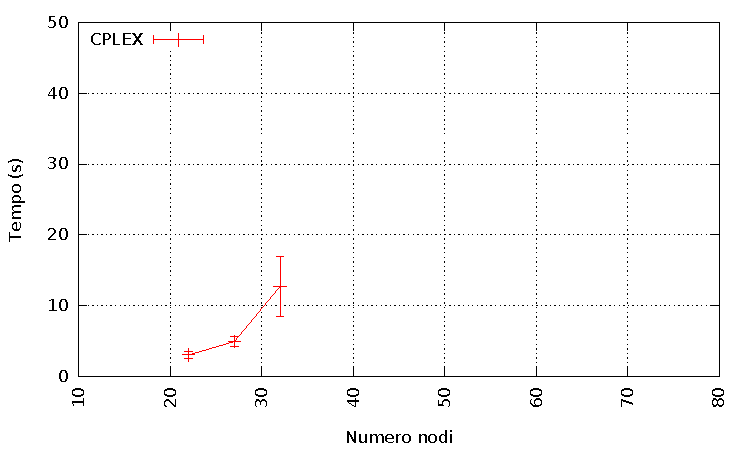
\includegraphics[width=\textwidth]{immagini/cplex_casuali.pdf}
		\caption{Istanze casuali}
		\label{fig:casuali cplex}
	\end{subfigure}
	\quad
	\begin{subfigure}[b]{.45\textwidth}
		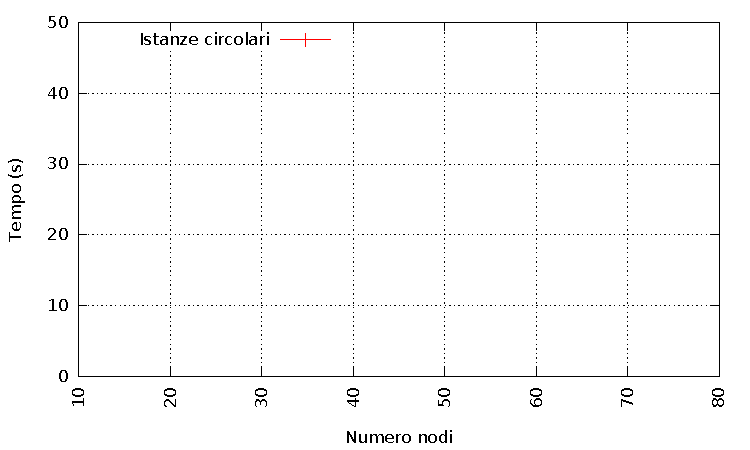
\includegraphics[width=\textwidth]{immagini/cplex_circolari.pdf}
		\caption{Istanze circolari}
		\label{fig:circolari cplex}
	\end{subfigure}
	\caption{Istanza casuali e circolari - \acronimo{cplex}}
	\label{fig:casuali circolari cplex}
\end{figure}

\begin{figure}[H]
	\centering
	\begin{subfigure}[b]{.45\textwidth}
		\includegraphics[width=\textwidth]{immagini/cplex_cluster_1.pdf}
		\caption{Istanze 1 cluster}
	\end{subfigure}
	\quad
	\begin{subfigure}[b]{.45\textwidth}
		\includegraphics[width=\textwidth]{immagini/cplex_cluster_2.pdf}
		\caption{Istanze 2 cluster}
	\end{subfigure}
	\\
	\begin{subfigure}[b]{.45\textwidth}
		\includegraphics[width=\textwidth]{immagini/cplex_cluster_3.pdf}
		\caption{Istanze 3 cluster}
	\end{subfigure}
	\quad
	\begin{subfigure}[b]{.45\textwidth}
		\includegraphics[width=\textwidth]{immagini/cplex_cluster_4.pdf}
		\caption{Istanze 4 cluster}
	\end{subfigure}
	\caption{Istanze cluster - \acronimo{cplex}}
	\label{fig:cluster cplex}
\end{figure}

\clearpage
\subsection{Tempi di risoluzione per \tabu}

\begin{figure}[H]
	\centering
	\begin{subfigure}[b]{.45\textwidth}
		\includegraphics[width=\textwidth]{immagini/tabu_4_tempo.pdf}
		\caption{Tenure 4}
	\end{subfigure}
	\quad
	\begin{subfigure}[b]{.45\textwidth}
		\includegraphics[width=\textwidth]{immagini/tabu_5_tempo.pdf}
		\caption{Tenure 5}
	\end{subfigure}
	\\
	\begin{subfigure}[b]{.45\textwidth}
		\includegraphics[width=\textwidth]{immagini/tabu_6_tempo.pdf}
		\caption{Tenure 6}
	\end{subfigure}
	\quad
	\begin{subfigure}[b]{.45\textwidth}
		\includegraphics[width=\textwidth]{immagini/tabu_7_tempo.pdf}
		\caption{Tenure 7}
	\end{subfigure}
	\\
	\begin{subfigure}[b]{.45\textwidth}
		\includegraphics[width=\textwidth]{immagini/tabu_8_tempo.pdf}
		\caption{Tenure 8}
	\end{subfigure}
	\caption{Tempi istanze casuali - \tabu}
	\label{fig:tempi tabu}
\end{figure}

\clearpage
\subsection{Costi delle soluzioni con \tabu}

\begin{figure}[H]
	\centering
	\begin{subfigure}[b]{.45\textwidth}
		\includegraphics[width=\textwidth]{immagini/tabu_4_costo.pdf}
		\caption{Tenure 4}
	\end{subfigure}
	\quad
	\begin{subfigure}[b]{.45\textwidth}
		\includegraphics[width=\textwidth]{immagini/tabu_5_costo.pdf}
		\caption{Tenure 5}
	\end{subfigure}
	\\
	\begin{subfigure}[b]{.45\textwidth}
		\includegraphics[width=\textwidth]{immagini/tabu_6_costo.pdf}
		\caption{Tenure 6}
	\end{subfigure}
	\quad
	\begin{subfigure}[b]{.45\textwidth}
		\includegraphics[width=\textwidth]{immagini/tabu_7_costo.pdf}
		\caption{Tenure 7}
	\end{subfigure}
	\\
	\begin{subfigure}[b]{.45\textwidth}
		\includegraphics[width=\textwidth]{immagini/tabu_8_costo.pdf}
		\caption{Tenure 8}
	\end{subfigure}
	\caption{Costi istanze casuali - \tabu}
	\label{fig:costi tabu}
\end{figure}

\clearpage
\section{Tabelle}
\label{sec:tabelle}

\subsection{Statistiche istanze casuali risolte con \acronimo{cplex}}

\begin{table}[H]
	\footnotesize
	\centering
	\caption{Tempi e costi istanze casuali - \acronimo{cplex}}
	\label{tab:casuali}
	\begin{tabular}{cS[table-format=3.4]S[table-format=2.4]S[table-format=2.1]}
	\toprule
	\multirow{2}*{Numero nodi} 	& {Tempo medio} & {Deviazione standard} & \multirow{2}*{Costo medio} \\
								& {(s)}			& {(s)} 				& \\
	\midrule
	11 & 0.2873   & 0.1057  & 56.3  \\
	16 & 0.8526   & 0.4813  & 64.9  \\
	20 & 1.5769   & 0.8246  & 71.4  \\
	25 & 3.4898   & 1.0368  & 78.9  \\
	29 & 7.3978   & 2.9413  & 82.3  \\
	34 & 26.8308  & 16.9291 & 89.5  \\
	38 & 46.9522  & 24.9913 & 93.8  \\
	43 & 103.9365 & 20.5338 & 98.4  \\
	47 & 140.9027 & 32.241  & 104.3 \\
	52 & 248.989  & 56.1847 & 108.9 \\
	\bottomrule
	\end{tabular}
\end{table}

\subsection{Statistiche istanze circolari risolte con \acronimo{cplex}}

\begin{table}[H]
	\footnotesize
	\centering
	\caption{Tempi e costi istanze circolari - \acronimo{cplex}}
	\label{tab:circolari}
	\begin{tabular}{cS[table-format=1.4]S[table-format=3.0]cS[table-format=1.4]S[table-format=3.0]}
	\toprule
	\multirow{2}*{Numero nodi} 	& {Tempo medio} & \multirow{2}*{Costo} 	& \multirow{2}*{Numero nodi} 	& {Tempo medio} & \multirow{2}*{Costo}\\
								& {(s)}			&  						& 								& {(s)}			&  \\
	\midrule
	8  & 0.0497  & 16  & 48 & 1.3179  & 96  \\
	12 & 0.1395  & 24  & 52 & 2.082   & 104 \\
	16 & 0.0889  & 32  & 56 & 1.872   & 112 \\
	20 & 0.2956  & 40  & 60 & 2.0974  & 120 \\
	24 & 0.4236  & 48  & 64 & 2.2927  & 128 \\
	28 & 0.2015  & 56  & 68 & 3.4218  & 136 \\
	32 & 0.5441  & 64  & 72 & 3.2282  & 144 \\
	36 & 0.8529  & 72  & 76 & 4.0914  & 152 \\
	40 & 1.979   & 80  & 80 & 6.1834  & 160 \\
	44 & 1.0726  & 88  & 84 & 10.9662 & 168 \\
	\bottomrule
	\end{tabular}
\end{table}

\clearpage
\subsection{Statistiche istanze cluster risolte con \acronimo{cplex}}

\begin{table}[H]
	\scriptsize
	\centering
	\caption{Tempi e costi istanze cluster - \acronimo{cplex}}
	\label{tab:cluster}
	\begin{tabular}{ccS[table-format=3.4]S[table-format=2.4]S[table-format=2.1]}
	\toprule
		& \multirow{2}*{Numero nodi} 	& {Tempo medio} & {Deviazione standard} & \multirow{2}*{Costo medio} \\
		&								& {(s)}			& {(s)} 				& \\
	\midrule
	\multirow{10}*{\begin{sideways}1 cluster\end{sideways}}
	& 2  & 0.0014 & 0.0003 & 9.4  \\
	& 4  & 0.0615 & 0.0398 & 16.6 \\
	& 5  & 0.0869 & 0.0497 & 18.7 \\
	& 7  & 0.1319 & 0.0748 & 21.3 \\
	& 8  & 0.1385 & 0.054  & 22.0 \\
	& 10 & 0.3189 & 0.0984 & 24.3 \\
	& 11 & 0.291  & 0.0789 & 26.3 \\
	& 13 & 0.4964 & 0.1699 & 26.8 \\
	& 14 & 0.4064 & 0.1722 & 27.6 \\
	& 16 & 0.6702 & 0.361  & 29.5 \\
	\midrule
	\multirow{10}*{\begin{sideways}2 cluster\end{sideways}}
	& 4  & 0.0699  & 0.0425  & 42.6 \\
	& 8  & 0.1691  & 0.0432  & 48.7 \\
	& 10 & 0.311   & 0.1089  & 52.4 \\
	& 14 & 1.0156  & 0.5453  & 56.0 \\
	& 16 & 1.8287  & 0.9     & 57.3 \\
	& 20 & 2.8166  & 2.0485  & 60.5 \\
	& 22 & 4.4575  & 1.4326  & 62.9 \\
	& 26 & 8.9421  & 7.465   & 64.9 \\
	& 28 & 10.8049 & 13.7156 & 66.7 \\
	& 32 & 34.9293 & 23.7068 & 69.7 \\
	\midrule
	\multirow{10}*{\begin{sideways}3 cluster\end{sideways}}
	& 6  & 0.1352   & 0.0386  & 42.5 \\
	& 12 & 0.5497   & 0.2289  & 54.2 \\
	& 15 & 1.339    & 0.8126  & 59.1 \\
	& 21 & 3.2067   & 1.5346  & 65.0 \\
	& 24 & 3.5545   & 1.8926  & 68.8 \\
	& 30 & 10.6001  & 7.6928  & 75.5 \\
	& 33 & 27.8225  & 14.2214 & 76.9 \\
	& 39 & 54.7645  & 22.6315 & 83.3 \\
	& 42 & 81.3233  & 21.5073 & 84.8 \\
	& 48 & 143.7259 & 30.8332 & 88.3 \\
	\midrule
	\multirow{10}*{\begin{sideways}4 cluster\end{sideways}}
	& 8  & 0.1833   & 0.0568   & 51.8  \\
	& 16 & 0.9478   & 0.4664   & 66.8  \\
	& 20 & 2.2219   & 1.0474   & 71.1  \\
	& 28 & 8.2337   & 5.1144   & 84.0  \\
	& 32 & 21.5946  & 15.4934  & 85.2  \\
	& 40 & 67.568   & 29.8094  & 95.6  \\
	& 44 & 112.8703 & 35.9209  & 99.3  \\
	& 52 & 218.7097 & 56.75    & 105.6 \\
	& 56 & 287.7982 & 62.408   & 110.5 \\
	& 64 & 590.3494 & 162.3353 & 116.9 \\
	\bottomrule
	\end{tabular}
\end{table}

\clearpage
\subsection{Statistiche istanze casuali risolte con \tabu}

\begin{table}[H]
	\tiny
	\centering
	\caption{Tempi e costi istanze casuali - \tabu}
	\label{tab:tabu}
	\begin{tabular}{ccS[table-format=1.4]S[table-format=1.4]S[table-format=3.3]S[table-format=1.4]}
	\toprule
		& \multirow{2}*{Numero nodi} 	& {Tempo medio} & {Deviazione standard} & \multirow{2}*{Costo medio} 	& \multirow{2}*{Deviazione standard} \\
		&								& {(s)}			& {(s)} 				& 								& \\
	\midrule
	\multirow{10}*{\begin{sideways}tabu tenure 4\end{sideways}}
		& 11 & 0.0034 & 0.0004 & 56.5    & 6.6767 \\
		& 16 & 0.01   & 0.002  & 65.57   & 4.7053 \\
		& 20 & 0.019  & 0.0035 & 71.85   & 5.4122 \\
		& 25 & 0.0504 & 0.018  & 80.835  & 4.1725 \\
		& 29 & 0.088  & 0.0147 & 84.995  & 5.4998 \\
		& 34 & 0.1307 & 0.0034 & 92.72   & 5.5882 \\
		& 38 & 0.1612 & 0.0031 & 97.23   & 6.1365 \\
		& 43 & 0.2039 & 0.0036 & 102.47  & 4.4306 \\
		& 47 & 0.2399 & 0.0059 & 108.955 & 5.7146 \\
		& 52 & 0.2951 & 0.0037 & 115.14  & 4.4514 \\
	\midrule
	\multirow{10}*{\begin{sideways}tabu tenure 5\end{sideways}}
		& 11 & 0.003  & 0.0003 & 56.3    & 6.5301 \\
		& 16 & 0.0084 & 0.0013 & 65.2    & 4.4201 \\
		& 20 & 0.0157 & 0.0017 & 71.7    & 5.1616 \\
		& 25 & 0.0521 & 0.02   & 81.325  & 4.5705 \\
		& 29 & 0.0859 & 0.0188 & 84.16   & 6.029  \\
		& 34 & 0.1318 & 0.0033 & 91.91   & 5.8659 \\
		& 38 & 0.1621 & 0.0041 & 97.67   & 6.5716 \\
		& 43 & 0.2043 & 0.0044 & 102.215 & 3.8482 \\
		& 47 & 0.2408 & 0.0053 & 108.145 & 5.308  \\
		& 52 & 0.2952 & 0.005  & 114.095 & 5.2285 \\
	\midrule
	\multirow{10}*{\begin{sideways}tabu tenure 6\end{sideways}}
		& 11 & 0.0035 & 0.0007 & 56.3   & 6.5301 \\
		& 16 & 0.009  & 0.0022 & 65.4   & 4.2103 \\
		& 20 & 0.0153 & 0.0019 & 71.6   & 5.1302 \\
		& 25 & 0.0273 & 0.0001 & 79.635 & 4.1977 \\
		& 29 & 0.0678 & 0.0246 & 84.655 & 6.4902 \\
		& 34 & 0.132  & 0.0035 & 92.17  & 5.5874 \\
		& 38 & 0.164  & 0.0032 & 96.535 & 6.1201 \\
		& 43 & 0.2068 & 0.0049 & 101.05 & 3.9816 \\
		& 47 & 0.2437 & 0.0049 & 108.23 & 5.1757 \\
		& 52 & 0.2991 & 0.0046 & 113.62 & 4.3767 \\
	\midrule
	\multirow{10}*{\begin{sideways}tabu tenure 7\end{sideways}}
		& 11 & 0.0033 & 0.0007 & 56.4    & 6.4759 \\
		& 16 & 0.0087 & 0.0016 & 65.4    & 4.7284 \\
		& 20 & 0.0159 & 0.0022 & 71.49   & 5.1444 \\
		& 25 & 0.0521 & 0.0213 & 80.26   & 4.1083 \\
		& 29 & 0.0946 & 0.0092 & 84.1    & 5.7843 \\
		& 34 & 0.1346 & 0.0031 & 91.885  & 5.9886 \\
		& 38 & 0.1644 & 0.0039 & 96.585  & 5.6948 \\
		& 43 & 0.21   & 0.0028 & 101.31  & 3.6964 \\
		& 47 & 0.2453 & 0.0041 & 108.095 & 4.4573 \\
		& 52 & 0.301  & 0.0043 & 113.055 & 4.9569 \\
	\midrule
	\multirow{10}*{\begin{sideways}tabu tenure 8\end{sideways}}
		& 11 & 0.0039 & 0.001  & 56.3    & 6.5301 \\
		& 16 & 0.0087 & 0.0013 & 65.22   & 3.9947 \\
		& 20 & 0.0169 & 0.0028 & 71.74   & 5.4139 \\
		& 25 & 0.0329 & 0.0079 & 79.56   & 4.0538 \\
		& 29 & 0.0928 & 0.0114 & 84.02   & 5.3384 \\
		& 34 & 0.1344 & 0.0028 & 91.535  & 5.6116 \\
		& 38 & 0.1674 & 0.0036 & 95.995  & 6.3374 \\
		& 43 & 0.2105 & 0.004  & 101.77  & 3.8731 \\
		& 47 & 0.2478 & 0.004  & 107.385 & 4.5974 \\
		& 52 & 0.3067 & 0.0028 & 112.68  & 4.5225 \\
	\bottomrule
	\end{tabular}
\end{table}

\clearpage
\subsection{Statistiche istanze cluster risolte con \tabu}

\begin{table}[H]
	\tiny
	\centering
	\caption{Tempi e costi istanze 1 cluster - \tabu}
	\label{tab:tabu cluster 1}
	\begin{tabular}{ccS[table-format=1.4]S[table-format=1.4]S[table-format=3.3]S[table-format=1.4]}
	\toprule
		& \multirow{2}*{Numero nodi} 	& {Tempo medio} & {Deviazione standard} & \multirow{2}*{Costo medio} 	& \multirow{2}*{Deviazione standard} \\
		&								& {(s)}			& {(s)} 				& 								& \\
	\midrule
	\multirow{10}*{\begin{sideways}tabu tenure 4\end{sideways}}
	& 2  & 0.0001 & 0.0    & 9.4    & 5.0721 \\
	& 4  & 0.0002 & 0.0    & 16.6   & 3.56   \\
	& 5  & 0.0005 & 0.0001 & 18.7   & 2.08   \\
	& 7  & 0.0011 & 0.0003 & 21.3   & 2.993  \\
	& 8  & 0.0017 & 0.0003 & 22.0   & 2.4279 \\
	& 10 & 0.0026 & 0.0006 & 24.3   & 3.2622 \\
	& 11 & 0.0037 & 0.0011 & 26.3   & 2.6178 \\
	& 13 & 0.0051 & 0.001  & 26.9   & 2.8636 \\
	& 14 & 0.0062 & 0.0016 & 27.6   & 2.0105 \\
	& 16 & 0.0082 & 0.0015 & 29.905 & 2.5529 \\
	\midrule
	\multirow{10}*{\begin{sideways}tabu tenure 5\end{sideways}}
	& 2  & 0.0001 & 0.0    & 9.4    & 5.0721 \\
	& 4  & 0.0002 & 0.0001 & 16.6   & 3.56   \\
	& 5  & 0.0004 & 0.0    & 18.7   & 2.08   \\
	& 7  & 0.0011 & 0.0003 & 21.3   & 2.993  \\
	& 8  & 0.0016 & 0.0004 & 22.0   & 2.4279 \\
	& 10 & 0.0026 & 0.0005 & 24.3   & 3.2622 \\
	& 11 & 0.0031 & 0.0006 & 26.5   & 2.6656 \\
	& 13 & 0.0058 & 0.0026 & 26.9   & 2.8636 \\
	& 14 & 0.0061 & 0.0021 & 27.6   & 2.0105 \\
	& 16 & 0.0085 & 0.0021 & 29.61  & 1.9167 \\
	\midrule
	\multirow{10}*{\begin{sideways}tabu tenure 6\end{sideways}}
	& 2  & 0.0001 & 0.0    & 9.4    & 5.0721 \\
	& 4  & 0.0002 & 0.0    & 16.6   & 3.56   \\
	& 5  & 0.0004 & 0.0001 & 18.7   & 2.08   \\
	& 7  & 0.001  & 0.0001 & 21.3   & 2.993  \\
	& 8  & 0.0015 & 0.0002 & 22.0   & 2.4279 \\
	& 10 & 0.0025 & 0.0003 & 24.3   & 3.2622 \\
	& 11 & 0.0035 & 0.0009 & 26.3   & 2.6178 \\
	& 13 & 0.0053 & 0.0012 & 26.8   & 2.858  \\
	& 14 & 0.0066 & 0.0017 & 27.6   & 2.0105 \\
	& 16 & 0.0089 & 0.0017 & 29.6   & 2.1126 \\
	\midrule
	\multirow{10}*{\begin{sideways}tabu tenure 7\end{sideways}}
	& 2  & 0.0001 & 0.0    & 9.4    & 5.0721 \\
	& 4  & 0.0003 & 0.0001 & 16.6   & 3.56   \\
	& 5  & 0.0004 & 0.0001 & 18.7   & 2.08   \\
	& 7  & 0.001  & 0.0    & 21.3   & 2.993  \\
	& 8  & 0.0018 & 0.0004 & 22.0   & 2.4279 \\
	& 10 & 0.0025 & 0.0005 & 24.3   & 3.2622 \\
	& 11 & 0.0032 & 0.0005 & 26.3   & 2.6178 \\
	& 13 & 0.0054 & 0.0009 & 26.8   & 2.858  \\
	& 14 & 0.0064 & 0.0013 & 27.6   & 2.0105 \\
	& 16 & 0.0089 & 0.0015 & 29.6   & 2.1126 \\
	\midrule
	\multirow{10}*{\begin{sideways}tabu tenure 8\end{sideways}}
	& 2  & 0.0001 & 0.0    & 9.4    & 5.0721 \\
	& 4  & 0.0002 & 0.0    & 16.6   & 3.56   \\
	& 5  & 0.0004 & 0.0    & 18.7   & 2.08   \\
	& 7  & 0.0013 & 0.0004 & 21.3   & 2.993  \\
	& 8  & 0.0016 & 0.0002 & 22.0   & 2.4279 \\
	& 10 & 0.0031 & 0.0009 & 24.3   & 3.2622 \\
	& 11 & 0.0035 & 0.0008 & 26.3   & 2.6178 \\
	& 13 & 0.0056 & 0.0015 & 26.8   & 2.858  \\
	& 14 & 0.006  & 0.0007 & 27.8   & 2.4192 \\
	& 16 & 0.0097 & 0.0026 & 29.5   & 2.0391 \\
	\bottomrule
	\end{tabular}
\end{table}



\end{document}